% CVPR 2025 Paper Template; see https://github.com/cvpr-org/author-kit

\documentclass[10pt,twocolumn,letterpaper]{article}

%%%%%%%%% PAPER TYPE  - PLEASE UPDATE FOR FINAL VERSION
% \usepackage{cvpr}              % To produce the CAMERA-READY version
\usepackage[review]{cvpr}      % To produce the REVIEW version
% \usepackage[pagenumbers]{cvpr} % To force page numbers, e.g. for an arXiv version

% Import additional packages in the preamble file, before hyperref
%
% --- inline annotations
%
\newcommand{\red}[1]{{\color{red}#1}}
\newcommand{\todo}[1]{{\color{red}#1}}
\newcommand{\TODO}[1]{\textbf{\color{red}[TODO: #1]}}
% --- disable by uncommenting  
% \renewcommand{\TODO}[1]{}
% \renewcommand{\todo}[1]{#1}



% It is strongly recommended to use hyperref, especially for the review version.
% hyperref with option pagebackref eases the reviewers' job.
% Please disable hyperref *only* if you encounter grave issues, 
% e.g. with the file validation for the camera-ready version.
%
% If you comment hyperref and then uncomment it, you should delete *.aux before re-running LaTeX.
% (Or just hit 'q' on the first LaTeX run, let it finish, and you should be clear).
\definecolor{cvprblue}{rgb}{0.21,0.49,0.74}
\usepackage[pagebackref,breaklinks,colorlinks,allcolors=cvprblue]{hyperref}

%%%%%%%%% PAPER ID  - PLEASE UPDATE
\def\paperID{*****} % *** Enter the Paper ID here
\def\confName{CVPR}
\def\confYear{2025}

%%%%%%%%% TITLE - PLEASE UPDATE
\title{Large-scale Synthetic Data Generation of Ocean Marker Buoys with Unreal Engine 5}

%%%%%%%%% AUTHORS - PLEASE UPDATE
\author{First Author\\
Institution1\\
Institution1 address\\
{\tt\small firstauthor@i1.org}
% For a paper whose authors are all at the same institution,
% omit the following lines up until the closing ``}''.
% Additional authors and addresses can be added with ``\and'',
% just like the second author.
% To save space, use either the email address or home page, not both
\and
Second Author\\
Institution2\\
First line of institution2 address\\
{\tt\small secondauthor@i2.org}
}

\begin{document}
\maketitle

\begin{abstract}
    The ABSTRACT is to be in fully justified italicized text, at the top of the left-hand column, below the author and affiliation information.
    Use the word ``Abstract'' as the title, in 12-point Times, boldface type, centred relative to the column, initially capitalized.
    The abstract is to be in 10-point, single-spaced type.
    Leave two blank lines after the Abstract, then begin the main text.
    Look at previous \confName abstracts to get a feel for style and length.
    \end{abstract}

\section{Introduction}

and discusses the method used for generating labels for the synthetic data. The paper also discusses the applications of the synthetic data, such as training object detection models. The paper concludes with a discussion of future work. 

The data produced should be as realistic as possible to ensure that the models trained on it are able to be applied to real world data. The method for achieving high fidelity data is discussed in \ref{sec:achieving_high_fidelity}.

\section{Literature Review}

The generation of synthetic data for machine learning tasks has taken place for many years. It takes place to save time, reduce risk and increase the scope of the data produced. One such study identified a benefit in generating synthetic data of car crashes for predicting dangerous vehicles, reducing the missed detection rate by 18.5\% compared to real data only models. \cite{Kim_Lee_Hwang_Suh_2019} 

However, synthetic data generation can often lead to data which is too clean looking and missing the imperfections of the real world, such as natural variation, deformation and clutter. \cite{Feng_2024_CVPR}

\section{Benefits of Synthetic Data Generation of Marker Buoys}

\subsection{Efficiency}

To test the efficiency of the pipeline, a total of 1000 images were generated. With an initial delay of 5 seconds to allow the simulation to properly load and with a time taken of 2 seconds per image, the total time taken to generate the images was 33 minutes and 25 seconds. This does not include the time taken to generate the environment or the buoys, which was carried out separately. Furthermore, running the python script to generate the labels takes only a few seconds. This is covered in more detail in section \ref{sec:mask_coordinates}.

At a resolution of 512x512, around 600MB in data was generated, consisting of images with varying backgrounds, camera positions, lighting and weather conditions. This method frees up time for researches to focus on other tasks such as building the environments and sourcing realistic 3D models and textures. 

\subsection{Vast Scope of Possible Scenarios}

Unreal Engine 5 allows for the creation of realistic environments in basically any setting, if one can source the correct assets. This allows for the generation of data which covers scenarios which might be difficult or impossible to capture in the real world. For example, it allows for the generation of data in dangerous conditions such as in a storm or natural disaster and inconvenient conditions such as specific times of day or year.

\section{Methodology}

\subsection{Introduction}

The synthetic data generation system was built using Unreal Engine 5.4 and Python 3.11. The two systems do not run in unison and require running once each to generate the data, first the Unreal Engine simulation and then the Python script. The Unreal Engine simulation generates the images and the Python script generates the labels. While Unreal Engine sports a powerful blueprint system, C++ code was mainly used to develop the system such as event sequencing \ref{sec:handling_concurrent_actions}, camera positioning \ref{sec:positioning_the_camera} and screenshot capture .

\subsection{Achieving High Fidelity} \label {sec:achieving_high_fidelity}

Aside from being an efficient method of generating synthetic data, the contents of the data can be completely controlled. Unlike content generated with some neural networks \cite{richter2021enhancingphotorealismenhancement}, there are no hallucinations to deal with and temporal consistency is maintained throughout the data.


\section{The Environment}

A benefit of using Unreal Engine 5 is the ability to create realistic and varied environments which can 


\subsection{The Water} \label {sec:the_water}

The water in the simulation is provided by Unreal Engine 5's Water plugin, more specifically the Water Body Ocean class. This water is simulated at interactive rates as a fluid, with the ability to simulate waves and the results of environment effects such as colour and lighting. With the fluid being simulated in real time, the water is able to be interacted with by actors in the scene, such as the buoys, as discussed in \ref{sec:the_buoys}.

Wave simulation is achieved through the use of a trochoidal or Gerstner wave function \cite{constantin2017gerstner}.

A terrain is required for fluid simulation.

\subsection{The Terrain}

Terrain, with the purpose of appearing in scenes (and not just as a requirement for fluid simulation as discussed in section \ref{sec:the_water}), was created using one of two methods.

Two methods were experimented with for creating the terrain. The first was to make use of assets available on the Unreal Engine marketplace, most notably the Megascans library \cite{QuixelMegascans}. This methods has the benefit of allowing the developer to create a realistic environment which can be travelled. However, a major downside is that assets often cost money and it can take a long time to create a realistic environment.

The second method was to use high dynamic range images (HDRI) to create the illusion of terrain, which normally provided a realistic sky too as a bonus. This method allowed for near instant creation of a realistic environment, giving the illusion of entire lakes with mountains in the background. However, the downside is that as the image is projected in a dome around a central point, moving even small distances away from the central point can cause the illusion to be broken. For this task, HDRI-based environments were suitable as the camera was moving only short distances around a static point.

\subsection{The Sky}

\begin{figure}[t]
    \centering
    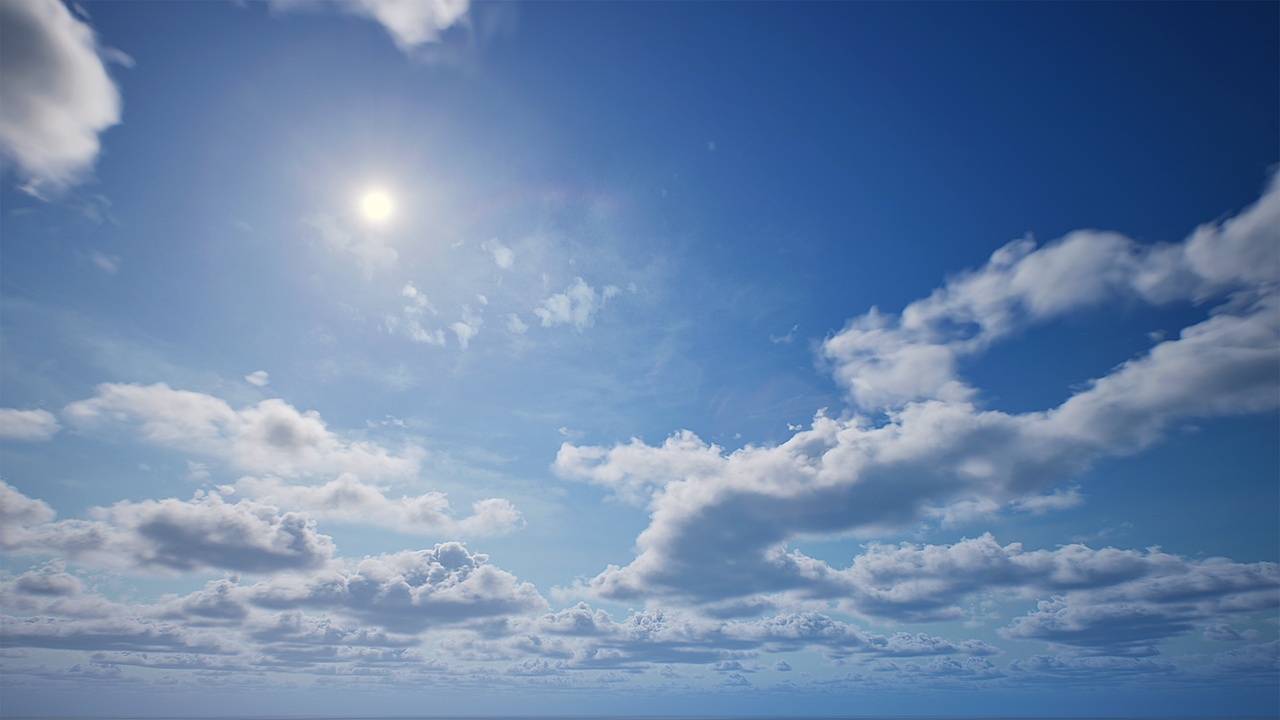
\includegraphics[width=\linewidth]{images/ultra_dynamic_sky.png}
    \caption{An example of the sky generated using the Ultra Dynamic Sky plugin in Unreal Engine 5.}
    \label{fig:sky_example}
\end{figure}

As with the terrain, two methods were experimented with for generating a realistic sky. The first was to use a plugin called Ultra Dynamic Sky \cite{UltraDynamicSky} which provided scene-wide realistic sky scapes and weather conditions. The second was to use a high dynamic range image (HDRI) to create the illusion of a sky. This method works well for static scenes in which minimal movement is required.

\subsection{The Weather}

Weather conditions, such as rain, snow and fog were also generated with the Ultra Dynamic Sky plugin, which includes a package called Ultra Dynamic Weather. As with the sky, this plugin allows for the generation of a range of weather scenarios which can be controlled. This was the only method used for generating weather conditions as it was the most efficient and realistic method found. Unlike with a HDRI, this method is not location specific and allows for weather simulation at any position within the scene.

\section{The Buoys}

\subsection{The Buoys} \label{sec:the_buoys}

The buoys are included in the scene as actors with static meshes, which play the part of digital twins of real marker buoys. The 3d models were purchased and imported into the scene. A class of MarkerBuoyBase was created which was inherited by all buoys in the scene. This class contained the logic for the buoys' behaviour.

Each buoy was placed in the scene at the same location to allow for the HDRI background to be effective, with all buoys apart from the subject of the current visit being set to invisible.

\subsection{Buoyancy}

Unreal Engine 5's water plugin allows for buoyancy simulation through the use of virtual pontoons. They act in the scene like invisible floatation aides and can be attached to objects allowing for fine tuning of the buoyancy of an object. The pontoons can be given X, Y and Z coordinates, relative to the object they are attached to, along with a buoyancy force.

For each buoy, 4 pontoons were placed at relative co-ordinates of:

\begin{itemize}

    \item X: 300, Y: 300, Z: 150
    \item X: 300, Y: -300, Z: 150
    \item X: -300, Y: -300, Z: 150
    \item X: -300, Y: 300, Z: 150 

\end{itemize}

\section{The Data Generation Pipeline}

\subsection{Introduction}

Having a realistic environment is great and can be a lot of fun to make. However, it does not achieve the end goal of this project. Actually having data which can be used to train models, with minimal input from users is the goal. This section discusses the pipeline, dubbed SyntheticDataGenerationSystem, which was a C++ class included as an actor in the scene and used to generate the data.

SyntheticDataGenerationSystem worked by looping through all of the actors in the scene which share the parent class of MarkerBuoyBase. The system effectively works by setting all buoys to the colour red \ref{sec:semantic_segmentation_masks}, hiding all of the buoys, positioning the camera randomly near the buoy and facing it, showing the buoy, taking a screenshot, changing its colour from red to its normal texture by changing its render pass in real time, taking a second screenshot and then hiding the buoy again. This process is repeated for each buoy in the scene. Once all of the images have been created, a Python script \ref{sec:mask_coordinates} is run which gets the coordinates of the outline of the buoy in the image and stores them in a .txt file.

\subsection{Handling Concurrent Actions} \label {sec:handling_concurrent_actions}

With the simulation being run in a video game engine, everything happens at interactive rates based on the frame rate of the simulation. Initially, a fundamental misunderstanding of how game engines work hindered progress. To summarise, as soon as the simulation began, all of the code written was executed in a single frame, causing n number of screenshots to be taken in an instant. The correct solution was to make use of Unreal Engine's Timer Handle (FTimerHandle) function, to schedule the taking of screenshots at a set interval.

To schedule the events, a cumulative delay was added to the timer handle in the form of:

cumulativeDelay = initialDelay + (markerBuoyNumber * numberOfVisits + visitNumber) * visitInterval;
 

\subsection{Positioning the Camera} \label {sec:positioning_the_camera}

To replicate the position of a camera as if it were on some sort of vessel, randomisation of the camera's position was included.

\subsection{Determining the Position of the Buoy}

Two methods for generating labels were tested. The first was to generate bounding boxes around the buoys in the scene using the inbuilt head's up display (HUD) feature. The second was to generate masks of the buoys in the scene. 

\subsection{Bounding Boxes}

Bounding boxes were generated by detecting points on the screen, per frame, which intersected with the buoy's static mesh. The bounding box was then generated by drawing a rectangle around the most northern, easter, southern and western points on the screen (see figure \ref{fig:buoy_with_bounding_box}). This method proved to be ineffective in generating tight bounding boxes around the buoys.

\begin{figure}[t]
    \centering
    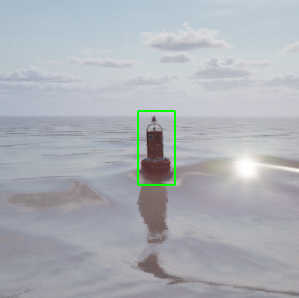
\includegraphics[width=\linewidth]{images/buoy_with_bounding_box.png}
    \caption{A buoy in the scene with a bounding box which is slightly too big.}
    \label{fig:buoy_with_bounding_box}
\end{figure}

\subsection{Semantic Segmentation Masks} \label {sec:semantic_segmentation_masks}

To set the buoys as a uniform and unique colour, Unreal Engine 5's Custom Depth feature was used. One can liken this to the layer feature in software such as Adobe Photoshop. This feature allows a static mesh to be rendered in a separate render pass, with this render pass (or "layer") having a separate material applied to it.  This feature was used to render the chosen buoy in just the colour red (RGB: 255, 0, 0).

\begin{figure}[t]
    \centering
    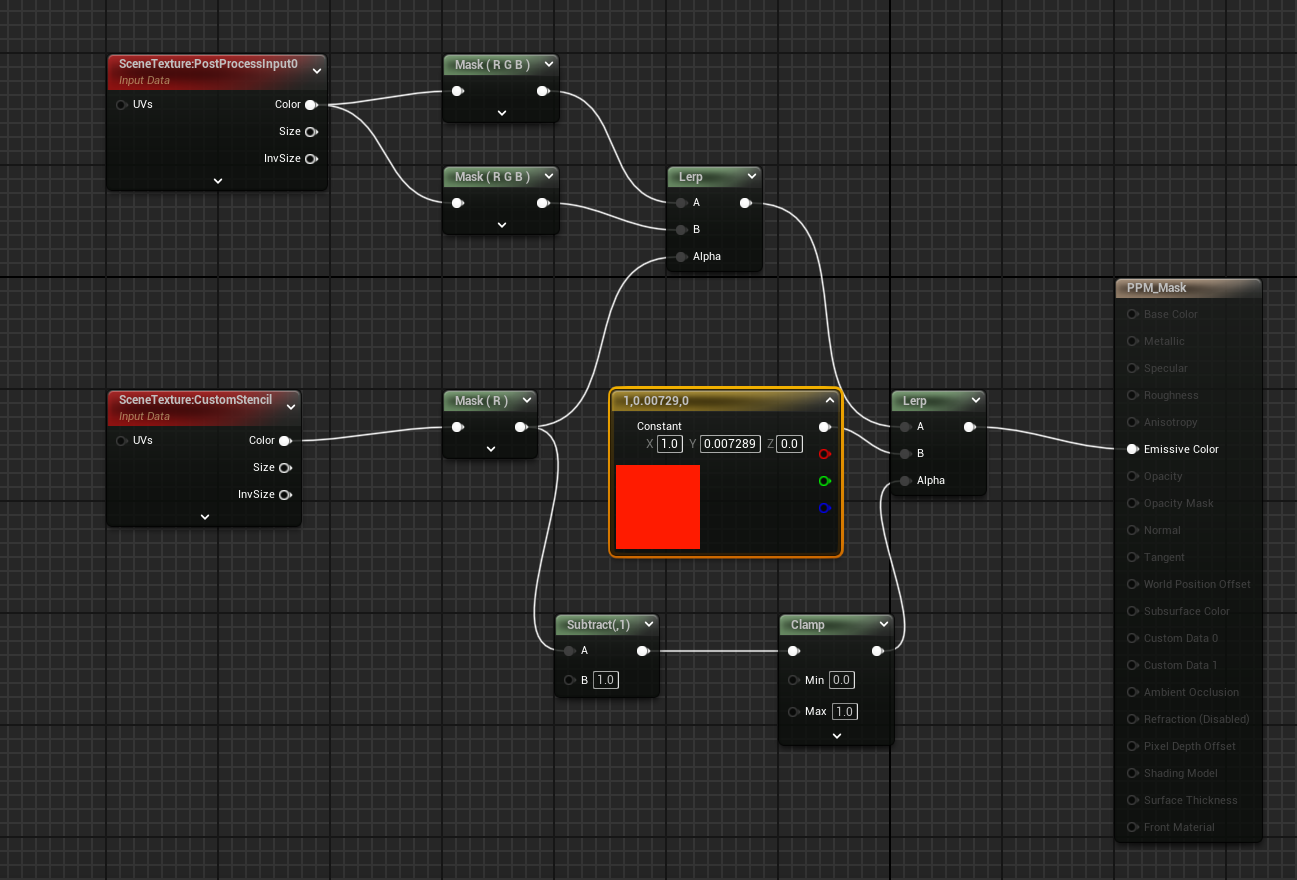
\includegraphics[width=\linewidth]{images/ppm_mask.png}
    \caption{An image of the blueprint used to generate the material for all objects in the chosen render pass.}
    \label{fig:ppm_mask}
\end{figure}

Inside the material, a Scene Texture node was added with a Scene Texture ID of PostProcessInput0, followed by the creation of a second Scene Texture node with a Scene Texture ID of CustomStencil.

The RGB values of the colour (color) output of PostProcessInput0 were connected to a Linear Interpolation node's A and B input values, with the R value (just red) of CustomStencil's colour output connected to the Alpha input of the Linear Interpolation node.

The R value of CustomStencil was also connected to a Subtract node's A input, with the B input set to 1.0. The output of the Subtract node was connected to a Clamp node with the Min set to 0.0 and the Max set to 1.0. The output of the Clamp node was then connected to the Alpha input of a second Linear Interpolation node.

A 3 Vector Constant node with its RGB values set to 1.0, 0.0, 0.0 was connected to the B input of the second Linear Interpolation node. The output of the first Linear Interpolation node was connected to the Alpha input of the second Linear Interpolation node. Finally, the output of the second Linear Interpolation node was connected to the Emissive Colour input of the material. This material should then be applied to every static mesh with a CustomDepth Stencil Value of 2.

\subsection{Automating Screenshot Capture}

By making use of FTimerHandle, as mentioned in \ref{sec:handling_concurrent_actions}, screenshots could be taken at set intervals. For each visit, two screenshots per buoy were taken, the first with the red semantic segmentation mask applied and the second without, with each being stored in separate directories. The position of the buoy was frozen for this so that the mask's coordinates perfectly matched that of the buoy in the unmasked image.

\subsection{Storing Mask Coordinates with a Python Script} \label {sec:mask_coordinates}

\begin{figure}[t]
    \centering
    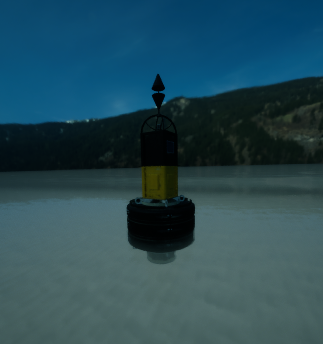
\includegraphics[width=\linewidth]{images/buoy_without_mask.png}
    \caption{A buoy in the scene without a mask.}
    \label{fig:buoy_without_mask}
\end{figure}

A Python script, dubbed Mask Pixel Joiner, was created. For each image inside the masked screenshot directory, the script would open the image and scan each row from left to right, until a red pixel was found. The script would then store the x and y coordinates of the red pixel. This would continue for every row of pixels. Once this was completed, the same process would be carried out but from bottom to top and right to left, determining the pixels which made up the edge of the buoy in an anti-clockwise direction. The coordinates were then stored in a .txt file.


\section{Applications}

The main application of this work is for generating data to train object detection models. 

\section{Conclusion}

In conclusion, this method for generating data is efficient and allows for scenarios to be catered for which might be difficult or impossible to capture in the real world. The data generated is of high fidelity and has high potential for use in training object detection models.

\section{Future Work}

Some sort of fail safe to ensure that the generation can recover if some issues occur such as a power cut.

{
    \small
    \bibliographystyle{ieeenat_fullname}
    \bibliography{main}
}

% WARNING: do not forget to delete the supplementary pages from your submission 
% \clearpage
\setcounter{page}{1}
\maketitlesupplementary


\section{Rationale}
\label{sec:rationale}
% 
Having the supplementary compiled together with the main paper means that:
% 
\begin{itemize}
\item The supplementary can back-reference sections of the main paper, for example, we can refer to \cref{sec:intro};
\item The main paper can forward reference sub-sections within the supplementary explicitly (e.g. referring to a particular experiment); 
\item When submitted to arXiv, the supplementary will already included at the end of the paper.
\end{itemize}
% 
To split the supplementary pages from the main paper, you can use \href{https://support.apple.com/en-ca/guide/preview/prvw11793/mac#:~:text=Delete%20a%20page%20from%20a,or%20choose%20Edit%20%3E%20Delete).}{Preview (on macOS)}, \href{https://www.adobe.com/acrobat/how-to/delete-pages-from-pdf.html#:~:text=Choose%20%E2%80%9CTools%E2%80%9D%20%3E%20%E2%80%9COrganize,or%20pages%20from%20the%20file.}{Adobe Acrobat} (on all OSs), as well as \href{https://superuser.com/questions/517986/is-it-possible-to-delete-some-pages-of-a-pdf-document}{command line tools}.

\end{document}
